\documentclass[12pt]{article}
\author{Lawrence Liu}
\usepackage{subcaption}
\usepackage{graphicx}
\usepackage{amsmath}
\usepackage{pdfpages}
\newcommand{\Laplace}{\mathscr{L}}
\setlength{\parskip}{\baselineskip}%
\setlength{\parindent}{0pt}%
\usepackage{xcolor}
\usepackage{listings}
%\definecolor{backcolour}{rgb}{0.95,0.95,0.92}
\usepackage{amssymb}
\usepackage[T1]{fontenc}
\usepackage{beramono}%\lstdefinestyle{mystyle}{
%    backgroundcolor=\color{backcolour}}
%\lstset{style=mystyle}
%\usepackage[usenames,dvipsnames]{xcolor}%%
%% Julia definition (c) 2014 Jubobs
%%



\title{ECE 133A HW 4}
\begin{document}
\maketitle
\section*{Exercise T13.3}
\subsection*{(a)}
With the following julia code we get:
\lstinputlisting[
    basicstyle=\tiny, %or \small or \footnotesize etc.
]{problem1.jl}
that 
$$\theta_1=3.125592633829346$$
and 
$$\theta_2=0.1540181798438225$$
which results in the following fit:\\
\includegraphics[scale=0.5]{"Moore's Law.png"}
\subsection*{(b)}
From our fit we expect the number of transistors to be:
$$10^{\theta_1+\theta_2(2015-1970)}\approx 10^{10}$$
Which is more than the acutally number of $4\cdot 10^9$ transistors:
\subsection*{(c)}
This is in line with Moore's law since
$2\theta_2=0.30803635968$ which is close to $\log_{10}(2)=0.30102999566$
\section*{Exercise T12.12}
\subsection*{(a)}
Let $p_{ik}=[u_{ik},v_{ik}]$ then we have that 
$$||p_{i_{1}}-p{j_{1}}||^2+\cdots+||p_{i_{L}}-p_{j_{L}}||^2=(u_{i_{1}}-u_{j_{1}})^2+\cdots+(u_{i_{L}}-u_{j_{L}})^2+(v_{i_{1}}-v_{j_{1}})^2+\cdots+(v_{i_{L}}-v_{j_{L}})^2$$
$$||p_{i_{1}}-p{j_{1}}||^2+\cdots+||p_{i_{L}}-p_{j_{L}}||^2=D(u)+D(v)$$
\subsection*{(b)}
Let C be the incident matrix of the graph we have that we want to minimize
$$||C^Tu||^2+||C^Tv||^2$$
Letting the matrix made up of the of the first $N-K$ rows of $C$
be the matrix $A$ and the last $K$ rows of $C$, likewise let
$u_{1}$ and $v_{1}$ be the first $N-K$ rows of $u$ and $v$ and
$u_{2}$ and $v_{2}$ be the last $K$ rows of $u$ and $v$ respectively, then we have
\begin{align*}
||B^Tu||^2+||B^Tv||^2&=||A^Tu_{1}+B^Tu_{2}||^2+||A^Tv_{1}+B^Tv_{2}||^2\\
&=\left|\left|\begin{bmatrix}
    A^T & 0\\
    0 & A^T
\end{bmatrix}\begin{bmatrix}
    u_{1}\\
    v_{1}
\end{bmatrix}+\begin{bmatrix}
    B^Tu_{2}\\
    B^Tv_{2}
\end{bmatrix}\right|\right|^2
\end{align*}
So then we have that in term of a least square problem we have
$||Ax-b||^2$
$$A=\begin{bmatrix}
    A^T & 0\\
    0 & A^T
\end{bmatrix}$$
And
$$b=\begin{bmatrix}
    B^Tu_{2}\\
    B^Tv_{2}
\end{bmatrix}$$
And
$$x=\begin{bmatrix}
    u_{1}\\
    v_{1}
\end{bmatrix}$$
\subsection*{(c)}
With the following code in julia
\lstinputlisting[
    basicstyle=\tiny, %or \small or \footnotesize etc.
]{problem2.jl}
We get the following plot:\\
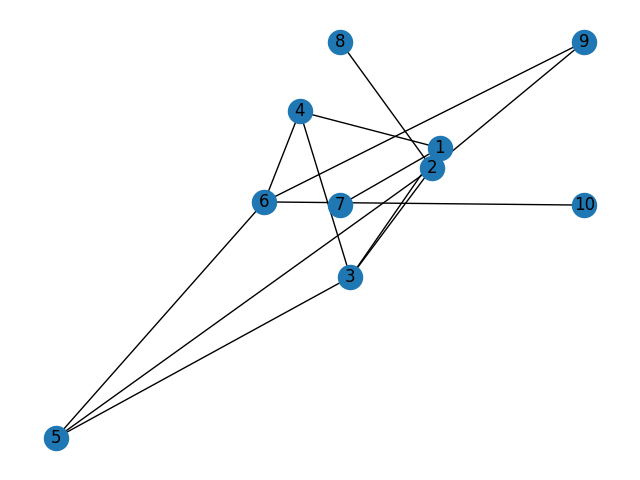
\includegraphics[scale=0.5]{fig1.png}
\section*{Exercise A8.3}
We can get that 
$$\alpha t_i+\beta=\ln(\frac{y_i}{1-y_i})$$
So therefore we can have a least squares problem, with
$$A=\begin{bmatrix}
t_1 & 1\\
t_2 & 1\\
\vdots & \vdots\\
t_n & 1
\end{bmatrix}$$
and 
$$b=[\ln(\frac{y_1}{1-y_1}),\ln(\frac{y_2}{1-y_2}),\dots,\ln(\frac{y_n}{1-y_n})]^T$$
and
$$x=[\alpha,\beta]^T$$
Then we have a least squares problem of 
$$||Ax-b||^2$$
To find $\alpha$ and $\beta$ I used the following code:
\lstinputlisting[
    basicstyle=\tiny, %or \small or \footnotesize etc.
]{problem3.jl}
which results in
$$\alpha=1.8676293241597044$$
$$\beta=-3.739673238861126$$
and the following fit:\\  
\includegraphics[scale=0.5]{"fig2.png"}
\section*{Exercise A5.11}
\subsection*{(a)}
we have that 
\begin{align*}
    x&=A^{\dagger}b\\
    x&=(A^TA)^{-1}A^Tb\\
    x&=\left(\begin{bmatrix}
        1 & 10^{-k} & 0\\
        1 & 0 & 10^{-k}
    \end{bmatrix}
    \begin{bmatrix}
        1 & 1\\
        10^{-k} & 0\\
        0 & 10^{-k}
    \end{bmatrix}\right)^{-1}
    \begin{bmatrix}
        1 & 10^{-k} & 0\\
        1 & 0 & 10^{-k}
    \end{bmatrix}
    \begin{bmatrix}
        -10^{-k}\\
        1+10^{-k}\\
        1-10^{-k}
    \end{bmatrix}\\
    x&=\left(\begin{bmatrix}
        1+10^{-2k} & 1\\
        1 & 1+10^{-2k}
    \end{bmatrix}\right)^{-1}\begin{bmatrix}
        10^{-2k}\\
        -10^{-2k}
    \end{bmatrix}\\
    x&=\begin{bmatrix}\frac{1+10^{-2k}}{10^{-4k}+2\cdot10^{-2k}}&-\frac{1}{10^{-4k}+2\cdot10^{-2k}}\\ -\frac{1}{10^{-4k}+2\cdot10^{-2k}}&\frac{1+10^{-2k}}{10^{-4k}+2\cdot10^{-2k}}
    \end{bmatrix}\begin{bmatrix}
        10^{-2k}\\
        -10^{-2k}
    \end{bmatrix}\\
    x&=\frac{10^{-2k}}{10^{-4k}+2\cdot10^{-2k}}\begin{bmatrix}
        2+10^{-2k}\\
        -2-10^{-2k}
    \end{bmatrix}
\end{align*}
thus we have for $k=6$:
$$x=\frac{10^{-12}}{10^{-24}+2\cdot10^{-12}}\begin{bmatrix}
    2+10^{-12}\\
    -2-10^{-12}
\end{bmatrix}$$
And for $k=7$ we have
$$x=\frac{10^{-14}}{10^{-28}+2\cdot10^{-14}}\begin{bmatrix}
    2+10^{-14}\\
    -2-10^{-14}
\end{bmatrix}$$
And for $k=8$ we have
$$x=\frac{10^{-16}}{10^{-32}+2\cdot10^{-16}}\begin{bmatrix}
    2+10^{-16}\\
    -2-10^{-16}
\end{bmatrix}$$
\subsection*{(b)}
We have that with the following code:
\begin{lstlisting}
for k = [6,7,8]

    A=transpose([[1,1] [10.0^-k,0] [0,10.0^-k]])
    b=[-(10.0^-k),1+10.0^-k, 1-10.0^-k]
    println("k=",k)
    println("x=",A\b)
    println("---------------------")
end
\end{lstlisting}
we get that 
\begin{verbatim}
k=6     
x=[0.9999999999176988, -0.999999999917699]
---------------------
k=7
x=[1.0000000027436178, -1.0000000027436176]
---------------------
k=8
x=[1.0000000043137076, -1.0000000043137076]
---------------------
\end{verbatim}
\subsection*{(c)}
We have that with the following code:
\begin{lstlisting}
for k = [6,7,8]

    A=transpose([[1,1] [10.0^-k,0] [0,10.0^-k]])
    b=[-(10.0^-k),1+10.0^-k, 1-10.0^-k]
    println("k=",k)
    println("x=",(A'*A) \ (A'*b))
    println("---------------------")
end
\end{lstlisting}
we get that
\begin{verbatim}
k=7
x=[1.0000000027436178, -1.0000000027436176]
---------------------
k=8
x=[1.0000000043137076, -1.0000000043137076]
---------------------
\end{verbatim}
And for $k=8$ we get a singular exception error since \verb +A'*A+ 
gets rounded to a matrix $\begin{bmatrix}
    1 & 1\\
    1 & 1
\end{bmatrix}$ that is singular
\section*{Exercise A5.12}
\subsection*{(a)}
$$f(y)=||Ay-b||^2+(c^Ty-d)^2$$
To minimize we take the derivative of it with respect to $y_i$ for all
$1\leq n \leq N$ and set it to zero have
$$\frac{\partial}{\partial y_i} f(y)=2(A^T(Ay-b))_i+2(c^Ty-d)c_i=0$$
Thus we have 
$$\nabla f(y)=2(A^T(Ay-b)+c(c^Ty-d))=0$$
which gives us
\begin{align*}
    \nabla f(y)&=0\\
    2(A^T(Ay-b)+c(c^Ty-d))&=0\\
    A^T(Ay-b)+c(c^Ty-d)&=0\\
\end{align*}
if $\hat{y}$ is a solution then we must have that
$$A^T(A\hat{y}-b)+c(c^T\hat{y}-d)=0$$
we can confirm this, since 
$$\hat{y}=\hat{x}+\frac{d-c^T\hat{x}}{1+c^T(A^TA)^{-1}c}(A^TA)^{-1}c$$
we have:
\begin{align*}
    A^T(A\hat{y}-b)+c(c^T\hat{y}-d)&=0\\
    A^TA\frac{d-c^T\hat{x}}{1+c^T(A^TA)^{-1}c}(A^TA)^{-1}c+cc^T\hat{x}+c(c^T\frac{d-c^T\hat{x}}{1+c^T(A^TA)^{-1}c}(A^TA)^{-1}c-d)&=0\\
    dc-c^T\hat{x}c+cc^T(d-c^T\hat{x})(A^TA)^{-1}c-c(d-c^T\hat{x})(1+c^T(A^TA)^{-1}c)&=0\\
    cc^T(d-c^T\hat{x})(A^TA)^{-1}c-c(d-c^T\hat{x})(c^T(A^TA)^{-1}c)&=0\\
    cc^T(d-c^T\hat{x})(A^TA)^{-1}c-cc^T(d-c^T\hat{x})(A^TA)^{-1}c&=0
\end{align*}
\subsection*{(b)}
We first compute the QR factorization fo $A$, which will cost us $2mn^2$ flops, 
then we can compute 
$\hat{x}$ with an additonal $2mn+n^2$ flops. Likewise,
since we can rewrite $(A^TA)^{-1}c$ as $(R^TQ^TQR)^{-1}c=(R^TR)^{-1}c$, which 
we can solve in $2n^2$ flops. then computing $c^T\hat{x}$ and $c^T(A^TA)^{-1}c$ will
each cost us an additional $2n-1$ flops, then computing $\frac{d-c^T\hat{x}}{1+c^T(A^TA)^{-1}c}$ will 
cost us 3 flops.Then computing $\hat{x}+\frac{d-c^T\hat{x}}{1+c^T(A^TA)^{-1}c}(A^TA)^{-1}c$
will cost us $2n$ flops, so in total this algorithm will cost us 
$\boxed{2mn^2+2mn+3n^2+6n-1}$ flops.




\end{document}
